\lettrine{I}{n this chapter}, we present and discuss the results that we obtained from the empirical performance investigation of the Fribourg construction. Our approach is to statistically evaluate and present the data in different ways that should make the relevant aspects of the results apparent. 

As mentioned, our main performance measure is the number of states of the complements that are produced by the tested constructions. However, we also consider the number of timeouts and memory excesses (based on the time and memory limits presented in Section~\ref{4_lmits}) and the execution times of the different constructions. Note that while the results of the first measure, complement size for a given automaton for a given construction, are definitive and repeatable, the results of the second measure are dependent on the implementation and the execution environment. That is, running the same tests with different implementatios in a different execution environment is likely to produce different results. This is why we take these runtime-dependent measure with care, and focus on the more robust measure of complement sizes.

Complement size means number of states of the complement.


Section~\ref{5_internal} presents the results of the internal tests, and Section~\ref{5_external} presents the results of the external tests. Both sections have two subsections. The first one for the results of the \goal{} test set, and the second one for the results of the Michel test set.

In Section~\ref{5_discussion} we summarise and discuss the most important results and insights gained from the study. Finally, in Section~\ref{5_limitations}, we identify the limitations of our study.


\section{Results of the Internal Tests}
\label{5_internal}
In the internal tests, we run different versions of the Fribourg construction on the \goal{} test set (see Section~\ref{4_goal_testset}), and the Michel test set (see Section~\ref{4_michel_testset}). 


The internal tests consists of the testing of different versions of the Fribourg construction with both, the \goal{} test set and the Michel test set (see Section~\ref{4_internal}). The tested construction versions differ for the two test sets. Below, we present the results of these two tests sets separately.

\subsection{GOAL Test Set}
\label{5_internal_goal}

For the \goal{} test set, the tested versions of the Fribourg construction are (see Section~\ref{4_internal}):
\begin{enumerate}
\item Fribourg
\item Fribourg+R2C
\item Fribourg+R2C+C
\item Fribourg+M1
\item Fribourg+M1+R2C
\item Fribourg+M1+R2C+C
\item Fribourg+M1+M2
\item Fribourg+R
\end{enumerate}

Below we present the results for all these eight versions from different perspectives. We first analyse the overall results, that is the results for the entire test set. Then, we analyse the results for each of the 110 transition density/acceptance density classes in which the \goal{} test set is divided into. Finally, we generalise these per-class results by trying to establish a categorisation of the \goal{} test set automata into \textit{easy}, \textit{medium}, and \textit{hard} automata.

\subsubsection{Overall Results}
First of all, we have to see how many timeouts and memory excesses there are in order to establish the effective samples, that is, the set of automata that have been successfully complemented by \textit{all} of the tested constructions.All the remaining analyses in this section are based on this set of effective samples. Table~\ref{i.g.out_table} shows the number of timeouts and memory excesses for each of the tested Fribourg construction versions.

\begin{table}[ht]
\centering
% latex table generated in R 3.1.2 by xtable 1.7-4 package
% Sat Jun  6 16:42:17 2015
\begin{tabular}{lrr}
  \hline
Construction & Timeouts & Memory excesses \\ 
  \hline
Fribourg & 48 & 0 \\ 
  Fribourg+R2C & 30 & 0 \\ 
  Fribourg+R2C+C & 54 & 0 \\ 
  Fribourg+M1 & 2 & 0 \\ 
  Fribourg+M1+M2 & 1 & 0 \\ 
  Fribourg+M1+R2C & 1 & 0 \\ 
  Fribourg+M1+R2C+C & 8 & 0 \\ 
  Fribourg+R & 48 & 0 \\ 
   \hline
\end{tabular}

\caption{Number of timeouts and memory excesses in the internal tests with the \goal{} test set.}
\label{i.g.out_table}
\end{table}

As can be seen in Table~\ref{i.g.out_table}, there is no memory excess for any of the construtions. That is, none of the constructions required more than 1 GB Java heap for any of the 11,000 complementation tasks in the \goal{} test set. However, as can be seen, there are some timeouts. For example, Fribourg, has 48 timeouts, which means that 48 of its complementation tasks were aborted, because they exceeded the time limit of 600 CPU time seconds per automaton.

Based on these results, we have to determine the effective samples, that is, the set of automata that have been successfully processed by \textit{all} the eight constructions. The analysis yields a set of effective samples of 10,939 automata. This means that 61 automata (0.55\%) are excluded because their complementation failed for at least one of the constructions. All the following analyses will be based on these 10,939 automata of the effective samples.

Having determined the effective samples, we can turn to the analysis of our main performance measure, namely the sizes of the produced complements. To get a first impression, in Figure~\ref{i.g.stripchart} we plot all the measured complement sizes in a stripchart. The complement sizes of all the tested constructions are represented as a strip containing a circle for each of the 10,939 automata of the effective samples. The number of states of the corresponding complements are indicated on the $x$-axis.

\begin{figure}[ht]
\centering
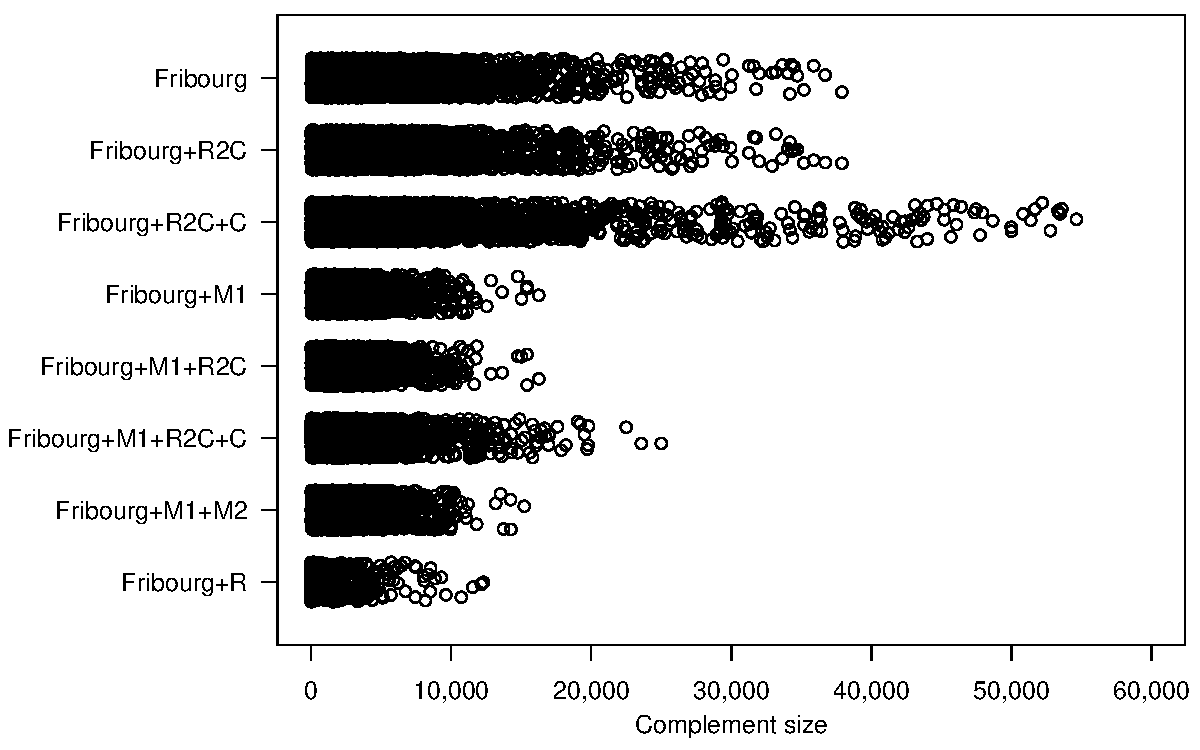
\includegraphics[width=0.7\textwidth]{figures/r/internal/goal/s.stripchart.pdf}
\caption{Complement sizes of the 10,939 effective samples for each tested version of the Fribourg construction on the \goal{} test set.}
\label{i.g.stripchart}
\end{figure}

The first thing to note is that the distribution of complement sizes is right-skewed (also known as positive-skewed). This means that there are many small complements, and then gradually fewer larger complements. This results in a long tail toward the right  on the $x$-axis. Generally, in right-skewed distributions, the mean is larger than the median, because the mean is increased by the few number of larger or extremely large values. We will see that this is the case for our complement size distribution further below.

The stripchart allows to intuitively compare the density of large complements that are produced by the different versions. Going from top to bottom, the distributions of Fribourg and Fribourg+R2C have similarly long tails. Fribourg+R2C+C, however, has a considerably longer tail. This shows us that the C option has a significant effect on the complement sizes, because it adds an additional state to the automata which are not complete. As we have seen in Section~\ref{4_goal_testset}, only 9\% of the automata of the \goal{} test set are alreacy complete. Thus 91\% of the automata are affected by the C option.

Next, Fribourg+M1, Fribourg+M1+M2, and Fribourg+M1+R2C all have similarly long tails. However, these tails are significantly shorter than the ones of the previous three versions. This indicates that the M1 optimisation is very effective in reducing the complement sizes.

Fribourg+M1+R2C+C again has a longer tail than Fribourg+M1+R2C. The reason for this is most likely the effect of the C option that we already observed for Fribourg+R2C and Fribourg+R2C+C.

Finally, Fribourg+R has the shortest tail of all versions. Fribourg+R is a special case, because it is the same construction as Fribourg, but with the difference that at the end of the constrcution, all unreachable and dead states are removed. Comparing the strips of Fribourg and Fribourg+R thus gives an idea of how many unreachable and dead states the Fribourg construction produces for the tested automata.

The stripchart in Figure~\ref{i.g.stripchart} gives a good first impression about the distribution of produced complement sizes of the different versions. However, for further insights, we need to statistically evaluate these distributions. Table~\ref{i.g.stats} shows the mean complement size for each version, along with the classical five-number summary consisting of the minimum value, 25th percentile, median, 75th percentile and maximum value.

\begin{table}[ht]
\centering
% latex table generated in R 3.1.2 by xtable 1.7-4 package
% Sat Jun  6 16:42:20 2015
\begin{tabular}{lrrrrrr}
  \hline
Construction & Mean & Min. & P25 & Median & P75 & Max. \\ 
  \hline
Piterman+EQ+RO & 209.6 & 1 & 38.0 & 80.0 & 183.0 & 20,349 \\ 
  Slice+P+RO+MADJ+EG & 949.4 & 2 & 120.0 & 396.0 & 1,003.0 & 41,081 \\ 
  Fribourg+M1+R2C & 1,017.3 & 2 & 153.0 & 452.0 & 1,134.0 & 37,068 \\ 
   \hline
\end{tabular}

\caption{Statistics of the complement sizes of the 10,939 effective samples for each tested version of the Fribourg construction on the \goal{} test set.}
\label{i.g.stats}
\end{table}

As can be seen in Table~\ref{i.g.stats}, the mean is for all constructions significantly higher than the median. This is typical for right-skewed distributions. Generally, the median is said to be more robust than the mean, because it is not affected by extreme values. For example, for the distribution $(1,2,3,4,5)$ the mean and the median are both 3. If this distribution happens to contain an extreme value, for example, $(1,2,3,4,1000)$, then the mean is increased to 202, while the median is still 3. Thus, the median better represents the ``typical'' values of a distribution, whereas the mean better reflects the effect of extreme values. Both aspects may be important for the analysis of the data at hand. For our own analyses, we will mainly focus on the median, because we are more interested in the ``typical'' behaviour of the tested constructions. However, we will always put the median in relation with the mean and the the other statistical indicators in Table~\ref{i.g.stats}.

The medians in Table~\ref{i.g.stats} include provide interesting insights. Regarding Fribourg and Fribourg+R2C, there is a decrease of the median complement size from 761 to 689. This is expectable because the R2C removes certain states from the complements of the complete input automata (although the complete input automata make up only 9\% of all automata).

Regarding Fribourg+R2C+C the median complement size drops significantly to 451. This is surprising insofar as Fribourg+R2C+C has the highest mean of all versions, and in the stripchart in Figure~\ref{i.g.stripchart}, it has the longest tail. Thus at first glance, Fribourg+R2C+C might look like the worst version. However, regarding the median, and also the 25th percentile, Fribourg+R2C+C belongs actually to the best versions. On the other hand, regarding the 75th percentile and the maximum, Fribourg+R2C+C has the highest of all values. A possible explanation for this is that the R2C+C option combination makes small complements smaller and large complements larger. We will further elaborate on this phenomenon when we analyse the complement sizes for each of the transition density/acceptance density classes below. 

Regarding Fribourg+M1 and Fribourg+M1+M2, the median of the former is lower than the median of the latter (482 against 496). The same applies to the 25th and 75th percentile. This means that the application of the M1 optimisation alone results in smaller complements than the application of the M1 and M2 optimsiations together. At first sight this is surprising, because Fribourg+M1+M2 has a lower worst-case complexity than Fribourg+M1 (see Section~\ref{3_optimisations}). However, as we already hinted at in Section~\ref{1_empirical} in the introductory chapter, a lower worst-case state complexity does not mean smaller complements in concrete cases. With the results of Fribourg+M1 and Fribourg+M1+M2 we have an empirical evidence for this claim. Note that the mean of Fribourg+M1+M2 is slightly lower than the mean of Fribourg+M1, which might result from the cases where Fribourg+M1 produces larger complements than Fribourg+M1+M2. However, regarding the median, 25t percentile, and 75th percentile values, we still see Fribourg+M1 as the more performant version for the \goal{} test set, as we have indicated in Section~\ref{4_internal}.

Fribourg+M1+R2C decreases the median of Fribourg+M1 from 482 to 447. Also the 25th and 75th percentile are decreased. This results from the removal of states that the R2C option allows for the 9\% of complete automata in the \goal{} test set.

Comparing Fribourg+M1+R2C with Fribourg+M1+R2C+C, we observe a similar phenonmenon as for Fribourg+R2C and Fribourg+R2C+C. The median and 25th percentile drop significantly, whereas the mean, 75th percentile, and maximum value increase. Again it seems that making the 91\% of incomplete automata preliminiarily complete (by the C option) in order to apply the R2C optimisation to all of them, has a very positive effect on some automata, but a negative effect on others.

Finally, the results of Fribourg+R make apparent that this version is a special case. The median is 1, and further analysis reveals that all complements up to the 61st percentile have a size of 1. This number coincides well with the 61.8\% of automata in the \goal{} test set that are universal (see Section~\ref{4_goal_test_set}). These universal automata indeed have a minimum complement consisting of a single non-accepting state (an empty automaton). It seems that whatever complement the Fribourg construction produces for these automata, the R option prunes all but one state. Even though universal automata are special cases, the results of Fribourg+R still give an idea about the number of unreachable and dead states that are produced by the Fribourg construction.

\subsubsection{Results by Transition Density/Acceptance Density Class}
Up to now, we looked at the results that are aggregated over the entire test set. This mixes together all the automata of the 110 transition density/acceptance density classes. In this part, we analyse the results for each of these 110 classes separately. The goal is to reveal how the constructions perform on automata with very different characteristics, and to reveal the relative differences between them.

Such class-based analysis means that there is not just one value per statistical indicator for each construction, but 110 values, one for each class. For example, for every tested construction there are 110 means, 110 medians, and so on. In order to be able to present this amount of data, we restrict ourselves to the median values of each class. As already mentioned, our main focus is on the median, because it best reflects the ``typical'' results. Consequently, all the reported values in the following are median values. 

The per-class median complement sizes result in a similar type of data that we encountered in the analysis of the complete, universal, and empty automata in the \goal{} test set in Section~\ref{4_goal_testset}. There, we presented this data in two forms, as matrices and as perspective plots. The advantage of matrices is that they show the explicit values, the advantage of perspective plots is that they better show the relative differences and the overall pattern. For the sake of brevity, we use only perspective plots in this chapter. However, we provide the matrices corresponding to all the perspective plots of this chapter in Appendix~\ref{app_matrices}.

Figures~\ref{i.g.persp_1} and~\ref{i.g.persp_2} show the perspective plots with the per-class median complement sizes for the eight tested Fribourg construction version. Note that looking at these perspective plots corresponds to looking at the corresponding matrix from the bottom right corner. We keep this orientation for all the perspective plots in this chapter. Note that this orientiation is different from the orientatio used for the perspective plots presenting the number of complete, universal, and empty automata of the \goal{} test set in Section~\ref{4_goal_testset}. The colours of the rectangles (called facets) in the perspective plots depend on the ``height'' of the plot at their four corners, and are chosen to draw an analogy with mountains.

\newcommand{\perspwidth}{0.475}

\begin{figure}[ht]
\centering
  \hfill
  \begin{subfigure}[t]{\perspwidth\textwidth}
  \centering
  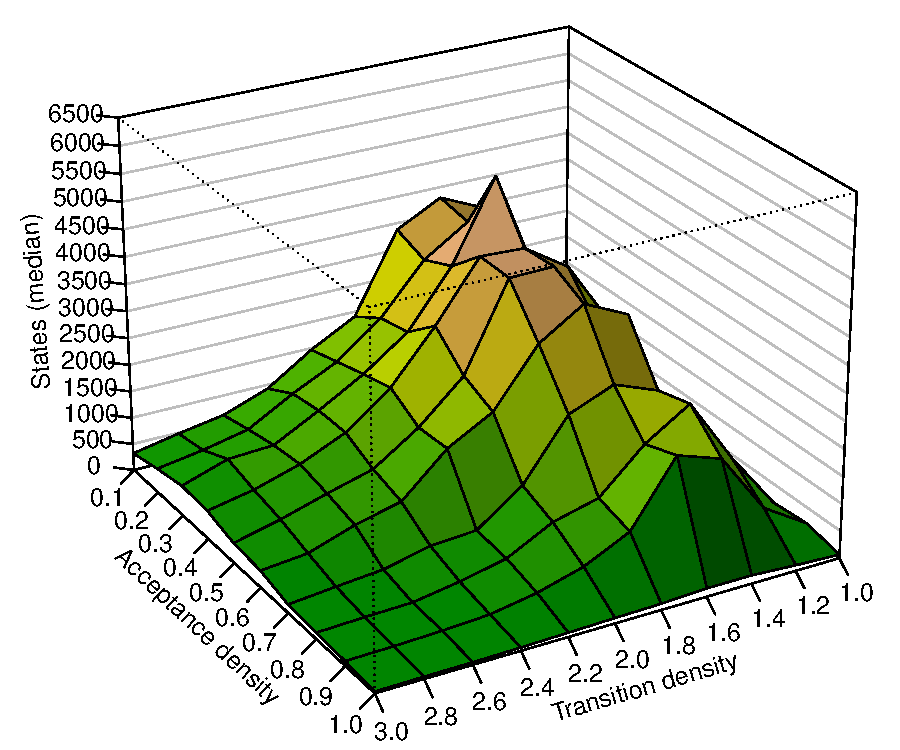
\includegraphics[width=\textwidth]{figures/r/internal/goal/s.median.Fribourg.pdf}
  \caption{Fribourg}
  \end{subfigure}
  \hfill
  \begin{subfigure}[t]{\perspwidth\textwidth}
  \centering
  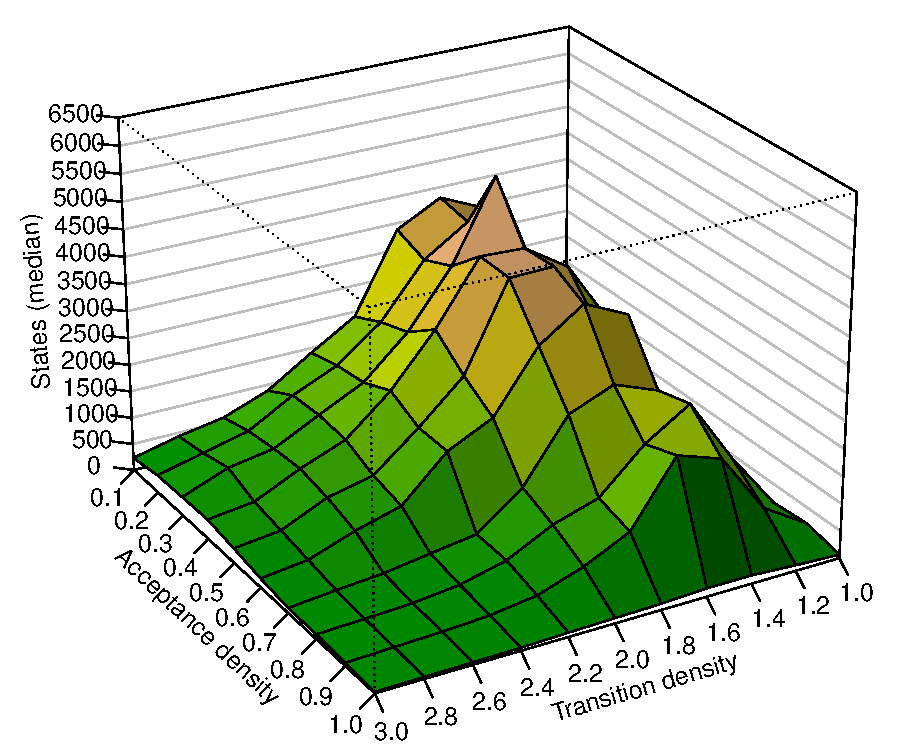
\includegraphics[width=\textwidth]{figures/r/internal/goal/s.median.Fribourg+R2C.pdf}
  \caption{Fribourg+R2C}
  \end{subfigure}
  \hfill

  \hfill
  \begin{subfigure}[t]{\perspwidth\textwidth}
  \centering
  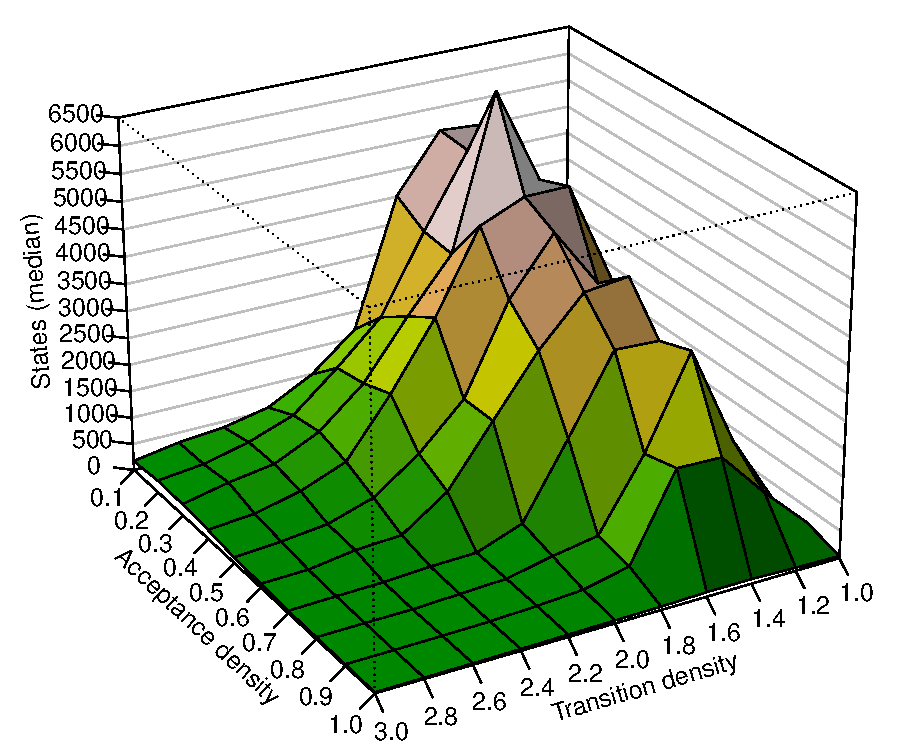
\includegraphics[width=\textwidth]{figures/r/internal/goal/s.median.Fribourg+R2C+C.pdf}
  \caption{Fribourg+R2C+C}
  \end{subfigure}
  \hfill
  \begin{subfigure}[t]{\perspwidth\textwidth}
  \centering
  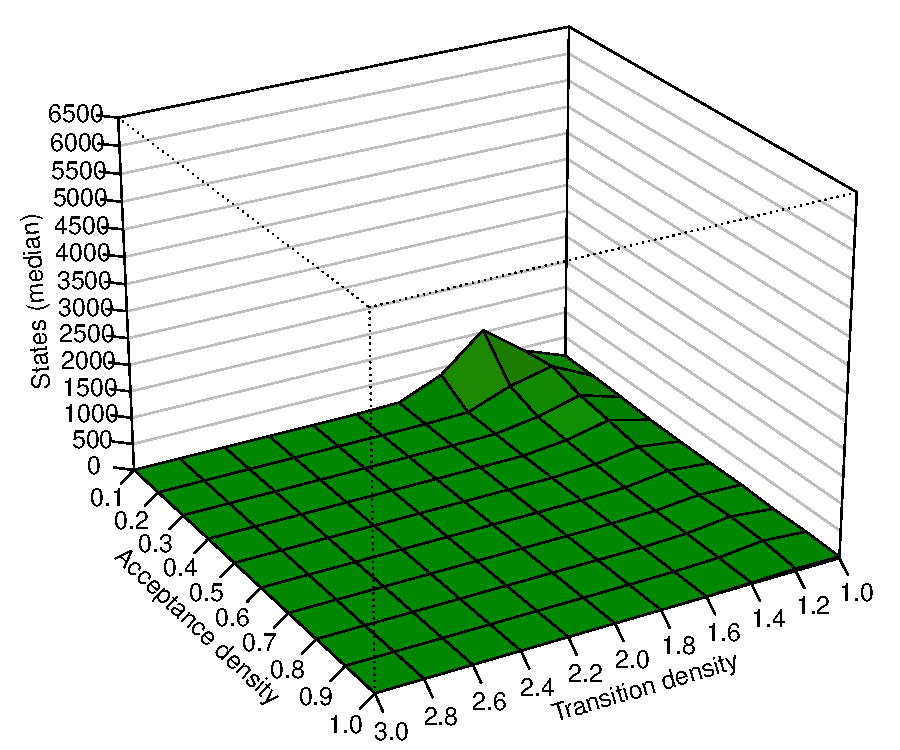
\includegraphics[width=\textwidth]{figures/r/internal/goal/s.median.Fribourg+R.pdf}
  \caption{Fribourg+R}
  \end{subfigure}
  \hfill  
\caption{Median complement sizes of the 10,939 effective samples for each of the 110 transition density/acceptance density classes of the \goal{} test set.}
\label{i.g.persp_1}
\end{figure}

As can be seen in the perspective plots of Figures~\ref{i.g.persp_1} and~\ref{i.g.persp_2}, there are large differences of the median complement sizes between the 110 transitio density/acceptance density classes. All constructions exhibit a mountain (in some it is only a hill) roughly in the area between transition densities of 1.2 and 2.4, and acceptance densities of 0.1 and 0.9. The mountain is oblong, and its ridge runs across the entire spectrum of acceptance densities. The summit of the ridge is roughly at a transition density of 1.6. In the direction of lower acceptance densities, the mountain keeps its high altitude. In the direction of higher acceptance densities, on the other hand, the mountain gradually flattens down until nearly ground level at an acceptance density of 1.0.

Comparing the height of the mountains in the perspective plots with the overall median complement sizes in Table~\ref{i.g.stats} might be surprising at first. The mountains have a height of roughly 2,000--5,000 states (except Fribourg+R), which corresponds to the median complement sizes of the corresponding classes. On the other hand, the overall median complement size of all construction is 761 states or less. However, a closer look at the perspective plots (and the corresponding matrices in Appendix~\ref{app_matrices}) reveals that around half of the classes have a rather low median complement size ($< 1,000$) what justifies the low overall median complement sizes in Table~\ref{i.g.states}. At the same time, this highlights the importance of a per-class analysis of the results on the \goal{} test set. It reveals much more accurately what to expect of the complementation of a specific automaton that resembles one of the classes of the \goal{} test set.

% Considering these median complement sizes in the perspective plots, apparently the automata of, for example, the class with a transition density of 1.6 and an acceptance density of 0.3 result in much larger complements than the automata of, for example, the class with a transition density of 3.0 and an acceptance density of 1.0. We could say that the automata of the first class are harder than the automata of the second class. Later in this section, we will try to identify hard, medium, and easy classes. For now, we will however focus on the relative differences between the different versions of the Fribourg construction.

Note that in the following, we will refer to specific points in the perspective plots in the form of coordinats $(t,a)$, where $t$ stands for the transition density, and $a$ for the acceptance density. For example, $(1.6,0.3)$ denotes the point at a transition density of 1.6 and an acceptance density of 0.3.

Let us now turn to the relative differences between the tested constructions. The plots of Fribourg and Fribourg+R2C in Figure~\ref{i.g.persp_1} (a) and (b) are rather similar. For both, the ridge has between 3,500 and 4,000 states with a peak of around 4,900 states at $(1.6, 0.3)$. In fact Fribourg+R2C only improves the performance on the complete input automata, compared to Fribourg. As we have analysed in Section~\ref{4_goal_testset}, the density of complete automata is highest in classes with high transition densities. By looking closely at the two plots, the values for the high transition density classes are indeed slightly lower for Fribourg+R2C than for Fribourg. Obviously, for classes that do not contain any complete automata, the values of the two constructions are identical.

Fribourg+R2C+C in Figure~\ref{i.g.persp_1} (c) has the highest mountain of all constructions. Its ridge has approximately 5,000 states, and it has a peak at $(1.6,0.3)$ of more than 6,000 states. This means basically that with Fribourg+R2C+C the ``mountain classes'' (the classes that result in large complements), result in even larger complements than for the other constructions. This might be surprising again, because as can be seen in Table~\ref{i.g.stats}, Fribourg+R2C+C has one of the lowest \textit{overall} median complement sizes. However, by comparing the classes with low median complement sizes of Fribourg+R2C+C with the other constructions, we see that they are indeed often even lower. This means that while the ``mountain classes'' have exceptionally high median complement sizes, the ``flatland classes'' have exceptionally low ones. This supports our previous proposition that the R2C+C combination, which includes the adding of a sink state to incomplete automata (which constitute 91\% of the \goal{} test set), makes easy complementation tasks easier and hard ones harder.


% an even higher mountain than the Fribourg and Fribourg+R2C. The top of the ridge is at around 5,000 states and the peak at the class 1.6/3.0 has close to 6,500 states. As already in the stripchart in Figure~\ref{i.g.stripchart}, Fribourg+R2C+C seems much worse than Fribourg+R2C at a first glance. However, as we have seen in Table~\ref{i.g.stats}, the median of Fribourg+R2C+C is 34.5\% lower than the median of Fribourg+R2C (689 to 451). By taking a closer look at the perspective plots of Fribourg+R2C and Fribourg+R2C+C, the reason for this can be seen. The low areas of Fribourg+R2C+C are slightly lower than the low areas of Fribourg+R2C. This is apparently enough to decrease the overall median. The much higher mountain peaks of Fribourg+R2C+C, on the other hand, do not influence the median. However, they show their effect in the overall mean which for Fribourg+R2C+C is 24\% higher than for Fribourg+R2C (2,424.6 to 1,955.9).

Fribourg+R in Figure~\ref{i.g.persp_1} (d) has, as expected, extremely low values for all the classes. In particular, 68 of the 110 classes have a median complement size of 1 (see corresponding matrix in Figure~\ref{i.g.matrices} (d) in Appendix~\ref{app_matrices}). We already hinted previously at the relation of a median complement size of 1 and the universal automata in the \goal{} test set. The per-class results of Fribourg+R reveal that all the classes with a median complement size of 1 contain 50 or more universal automata (compare matrices in Figure~\ref{i.g.matrices} (d) in Appendix~\ref{app_matrices} and Figure~\ref{testset_analysis} (b)). If all these univeral automata are reduced by the R option to a single-state automaton, then it explains the observed median complement size of 1 for these classes (remember that there are 100 automata in each class). However, also the classes which contain less than 50 universal automata have significantly lower complement median sizes than in the Fribourg construction without the R option. This indicates that the Fribourg construction also  generates numerous unreachable and dead states for non-universal automata. 

% Comparing the fourth plot in Figure~\ref{i.g.persp_1}, Fribourg+R, to the plots of Fribourg, Fribourg+R2C, and Fribourg+R2C+C is like comparing a Dutch polder to the Swiss Alps. The mountain shrinks to a small hillock and the rest of the terrain is low and flat. This is because so many complements of the Fribourg construction can be reduced to very small sizes by removing their unreachable and dead states. The corresponding matrix in Appendix~\ref{app_matrices} reveals that 68 of the 110 classes have a median complement size of 1. If we further compare this matrix to the matrix with the number of universal automata in Figure~\ref{testset_analysis} (b) in Section~\ref{4_goal_testset}, we see that all the classes with a median of 1 contain more than 50 universal automata, and the classes with a median greater than 1 contain less than 50 universal automata. There is a total of 100 automata per class. This makes sense as the complements of universal automata are empty automata, and every empty automaton can be reduced to an automaton with a single non-accepting state. Looking at the classes with a median greater than 1, we see that their values are still considerably lower than the ones of the plain Fribourg construction.

\begin{figure}[ht]
\centering
  \hfill
  \begin{subfigure}[t]{\perspwidth\textwidth}
  \centering
  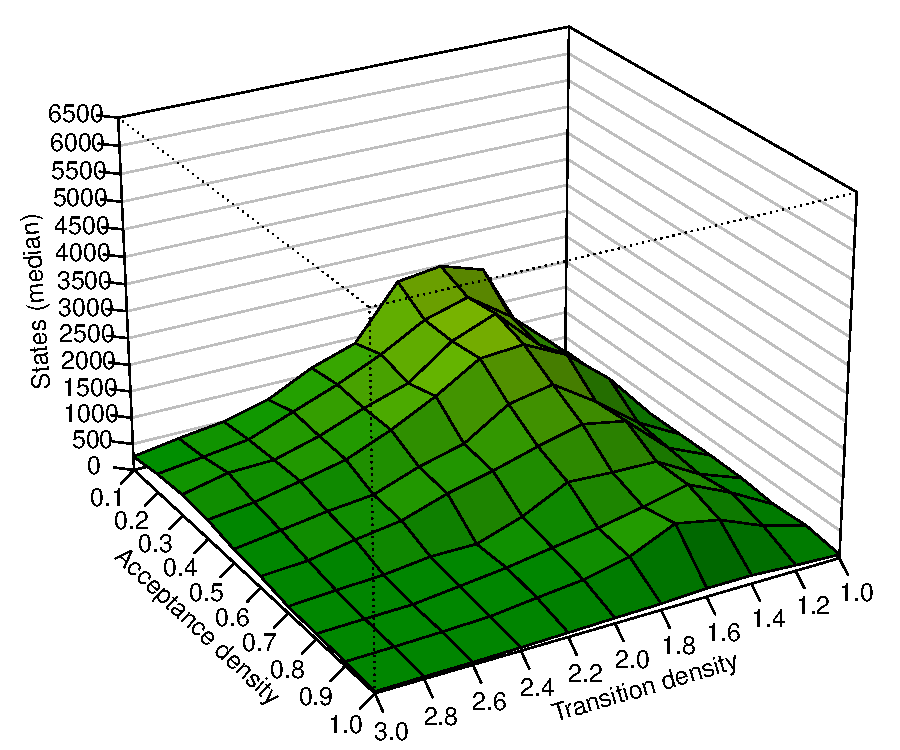
\includegraphics[width=\textwidth]{figures/r/internal/goal/s.median.Fribourg+M1.pdf}
  \caption{Fribourg+M1}
  \end{subfigure}
  \hfill
  \begin{subfigure}[t]{\perspwidth\textwidth}
  \centering
  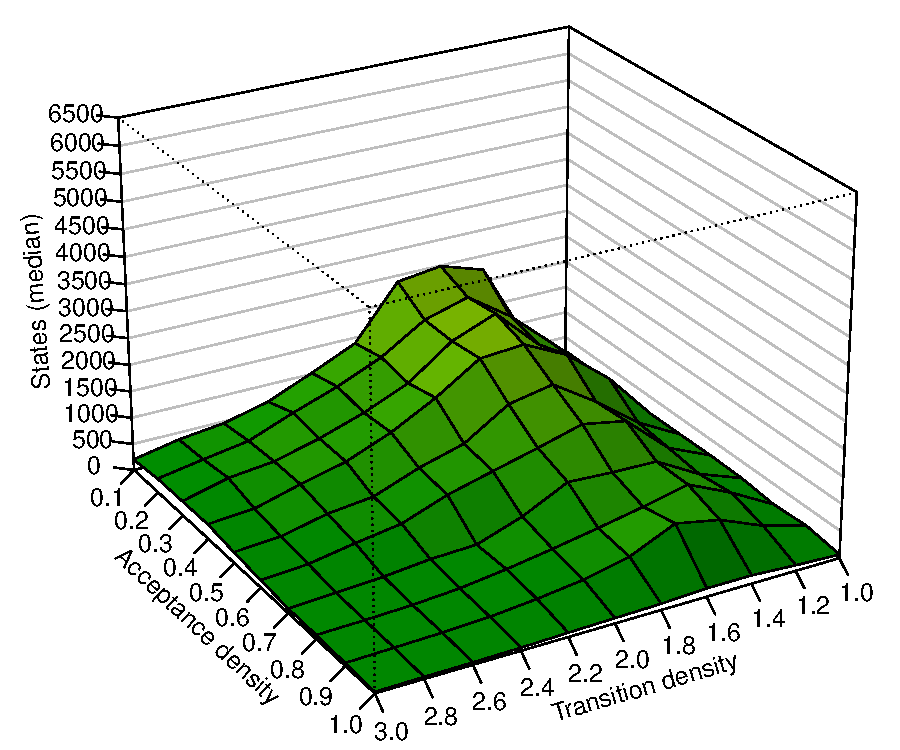
\includegraphics[width=\textwidth]{figures/r/internal/goal/s.median.Fribourg+M1+R2C.pdf}
  \caption{Fribourg+M1+R2C}
  \end{subfigure}
  \hfill

  \hfill
  \begin{subfigure}[t]{\perspwidth\textwidth}
  \centering
  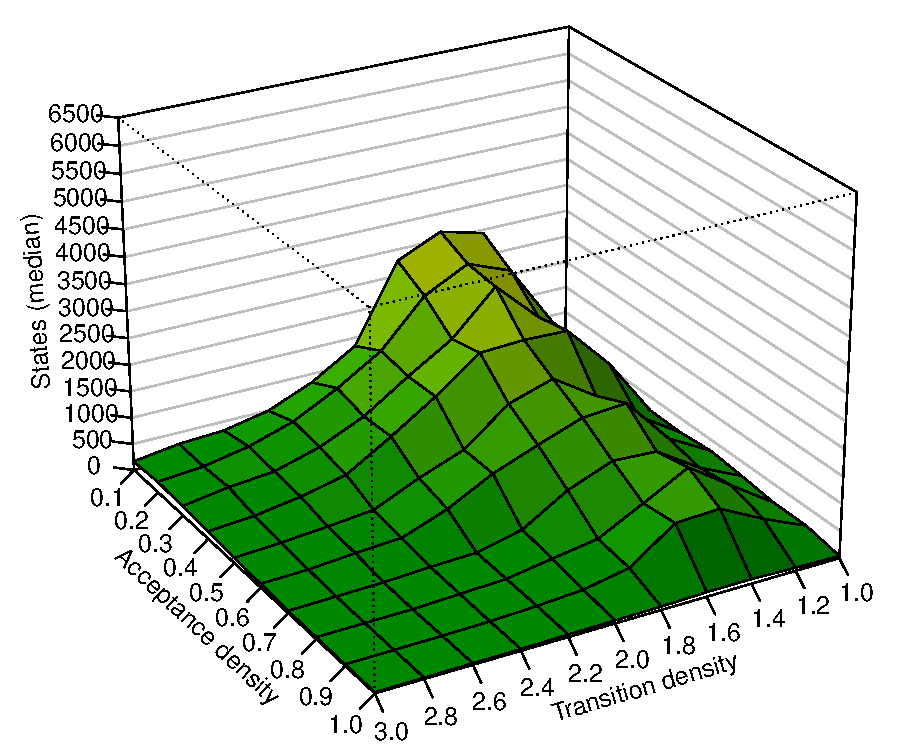
\includegraphics[width=\textwidth]{figures/r/internal/goal/s.median.Fribourg+M1+R2C+C.pdf}
  \caption{Fribourg+M1+R2C+C}
  \end{subfigure}
  \hfill
  \begin{subfigure}[t]{\perspwidth\textwidth}
  \centering
  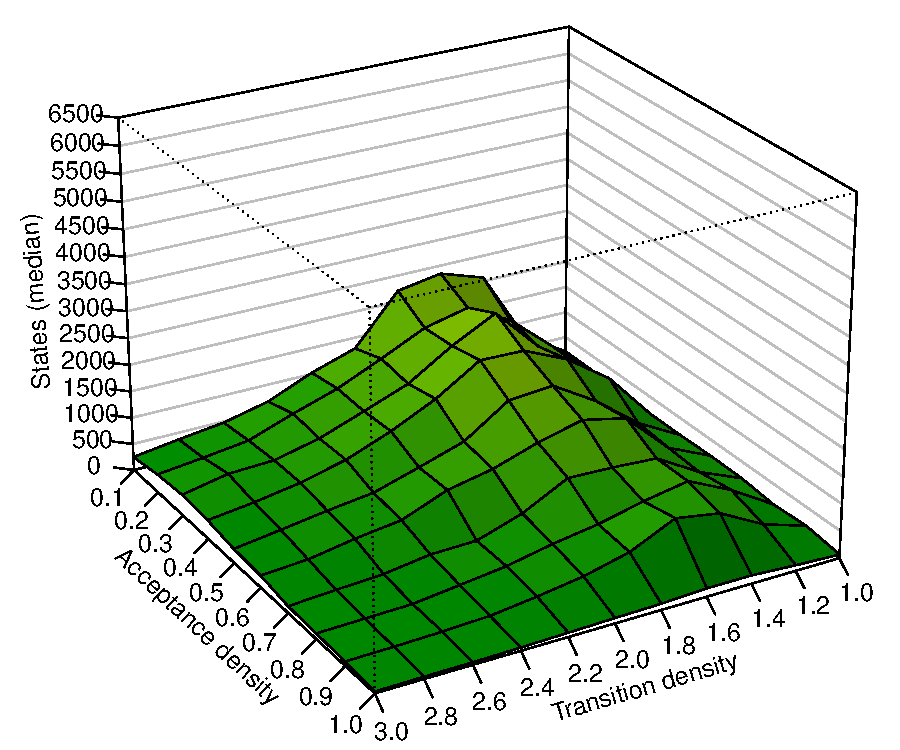
\includegraphics[width=\textwidth]{figures/r/internal/goal/s.median.Fribourg+M1+M2.pdf}
  \caption{Fribourg+M1+M2}
  \end{subfigure}
  \hfill
\caption{Median complement sizes of the 10,939 effective samples for each of the 110 transition density/acceptance density classes of the \goal{} test set.}
\label{i.g.persp_2}
\end{figure}

Figure~\ref{i.g.persp_2} shows the perspective plots for Fribourg+M1, Fribourg+M1+R2C, Fribourg+M1+R2C+C, and Fribourg+M1+M2. All of these versions include the M1 optimisation. The first three versions, Fribourg+M1, Fribourg+M1+R2C, and Fribourg+M1+R2C+C can be seen as pairs to Fribourg, Fribourg+R2C, and Fribourg+R2C+C, that additionally include the M1 optimisation. Most apparent by comparing these three pairs is that for the versions including M1 the mountain is significantly flatter. For Fribourg+M1 and Fribourg+M1+R2C the ridge has less than 2,500 states, as opposed to around 3,500 states for Fribourg and Fribourg+R2C. For Fribourg+M1+R2C+C the top of the ridge has around 3,000 states, as opposed to 5,000 states for Fribourg+R2C+C. This shows that the M1 optimisation causes a significant improvement for the automata of the ``mountain classes'', that is, the automata that generally result in larger complements. However, the M1 optimisation also has a positive effect on the automata of the ``flatland classes'', that is, the automata that typically result in smaller complements. This can be best seen in the corresponding matrices in Appendix~\ref{app_matrices}, or by comparing the overall means and  medians of the corresponding constructions with and without the M1 optimisation (see Table~\ref{i.g.stats}).

The relative differences between Fribourg+M1, Fribourg+M1+R2C, Fribourg+M1+R2C+C are very similar to the relative differences between Fribourg, Fribourg+R2C, and Fribourg+R2C+C. Also the reasons for these differences are basically the same, and caused by the R2C and C options, as we have previously explained for Figure~\ref{i.g.persp_1}.

Regarding Fribourg+M1+M2 in Figure~\ref{i.g.persp_2} (d), it is most interesting to compare it to Fribourg+M1, in order to isolate the effect of the M2 optimisation. From Table~\ref{i.g.stats}, we know that the overall median of Fribourg+M1+M2 is higher than the one of Fribourg+M1 (496 against 482), and the overall mean of Fribourg+M1+M2 is lower than the one of Fribourg+M1 (958.0 against 963.2). Comparing the per-class medians in the perspective plots of the two constructions does not reveal any salient differences, except that the highest values of Fribourg+M1+M2 seem to be slightly lower than the ones of Fribourg+M1. However, comparing the matrices of the two constructions in Figure~\ref{i.g.matrices} (e) and (h) reveals that Fribourg+M1+M2 has lower median complement sizes for almost all classes with acceptance densities between 0.1 and 0.4. On the other hand, Fribourg+M1+M2 has higher median complement sizes for most classes with an acceptance density between 0.5 and 0.9. Thus, the M2 optimsiation indeed has a positive effect on the performance, but only on \textit{some} automata. These automata are those that contain not too many accepting states. On the other hand, for automata with 50\% or more accepting states, the M2 optimisation decreases the performance, rather than increasing it. For many complementation constructions, automata with few accepting states are harder to complement than automata with a lot of accepting states ~\cite{2011_tsai}. This means that the M2 optimisation is especially suitable for these automata that are hard for other constructions. This makes it interesting to apply this optimisation selectively on automata on which a positive effect is expected.

 % of the remaining four versions of the Fribourg construction, all of which include the M1 optimisation. Most apparent in these plots is that the mountain that we described for the plots of Fribourg, Fribourg+R2C, and Fribourg+R2C+C is still there, but it is rather a hill than a mountain. For Fribourg+M1, and Fribourg+M1+R2C, the height of the ridge is around 2,500 states. This is reflected by the overall means of these two versions compared to their counterparts without the M1 optimisation, Fribourg, and Fribourg+R2C. The decrease of the overall mean from Fribourg to Fribourg+M1 is by 52\% (from 2004.6 to 963.2) and from Fribourg+R2C to Fribourg+M1+R2C by 52.1\% (from 1955.9 to 937.7). The decreases of the overall medians are by 36.6\% (from 761 to 482), and 35.1\% (from 689 to 447) for the same two pairs of versions. With this we can confirm that the M1 optimisation brings a significant performance gain for the automata in the \goal{} test set.

% Regarding the M2 optimisation, we can see that the mountain ridge in the Fribourg+M1+M2 perspective plot is slightly lower than the one in the Fribourg+M1 perspective plot. The flatland regions, however, seem to not change much. This is reflected by the overall mean of Fribourg+M1+M2 which is slightly lower than in Fribourg+M1 (958.9 opposed to 963.2). The overall median, on the other hand, is higher for Fribourg+M1+M2 than for Fribourg+M1 (496 opposed to 482). An interpretation of this behaviour is that the application of the M2 optimisation results in smaller complements for \textit{some} input automata. \textcolor{red}{Better analysis: Fribourg+M1+M2 is better for almost all classes with an acceptance density up to 0.4, and worse for most of the classes with a n acceptance density between 0.5 and 0.9. The results are exactly identical for all the classes with an acceptance density of 1.0!}. \textcolor{gray}{These automata are especially the hard ones that produce large complements. This positive effect of M2 does however not affect enough input automata, especially not the easy automata, as to improve the overall performance of the construction in terms of the median complement sizes. As already stated previously, we consider therefore Fribourg+M1 as the better construction on the \goal{} test set than Fribourg+M1+M2.}

% Finally,Fribourg+M1+R2C+C differs from Fribourg+M1+R2C in a similar way that Fribourg+R2C+C differs from Fribourg+R2C. The higher regions get higher and the lower regions get lower, that is, a performance decline on hard automata, but a performance gain on easy automata. The performance gain on the easy automata is however effective enough to decrease the overall median from 447 to 331, which is minus 26\%.

% With 331 states, Fribourg+M1+R2C+C has the lowest median of all the versions (apart from the special case Fribourg+R). However, we still declare Fribourg+M1+R2C as the winner on the \goal{} test set, mainly for two reasons. First, while Fribourg+M1+R2C+C has a lower median, the mean is still higher (1062.6 to 937.7 which is a plus of 13.3\%). This results from the complements of the hard automata, which are larger than with Fribourg+M1+R2C. From a practical point of view, the mean might be relevant, because it relates more directly to the required computing resources than the median. Indeed, the execution per complementation task in CPU time is 25.4\% higher for Fribourg+M1+R2C+C than for Fribourg+M1+R2C (all measured execution time in CPU time are presented in Appendix~\ref{app_times}). The increase in the average execution time per automaton is from 4.44 to 5.57 seconds and in the total execution time from 48,572 seconds ($\approx$ 135 hours) to 60,919 seconds ($\approx$ 169 hours). Fribourg+M1+R2C, on the other hand, has the lowest mean of all versions. The second reason that we choose Fribourg+M1+R2C as the winner and not Fribourg+M1+R2C+C is that the C option is not a real part of the construction. It actually modifies the input automata before the construction starts in order to make them better suited for the construction. Fribourg+M1+R2C, on the other hand, includes only construction-specific options.

\subsubsection{Difficulty Categories}
The per-class analysis shows that there are big difference in the complement sizes across the transition density/acceptanc density classes of the \goal{} test set. Furthermore, there is a certain pattern throughout the results of all construction, namely the mountain and the flatland regions. In the following, we attempt to categorise the classes of the \goal{} test set into \textit{easy}, \textit{medium}, and \textit{hard} categories. 

To this end, we calculated for each transition density/acceptance density class the average of the median complement sizes of all the tested constructions. This results in a matrix containing the average median complement sizes for each class. Then, we defined two breakpoints at 500 and at 1,600 states that divide the classes into easy, medium, and hard ones. The result of this analysis is shown in Figure~\ref{i.g.difficulty}.

\begin{figure}[ht]
\centering
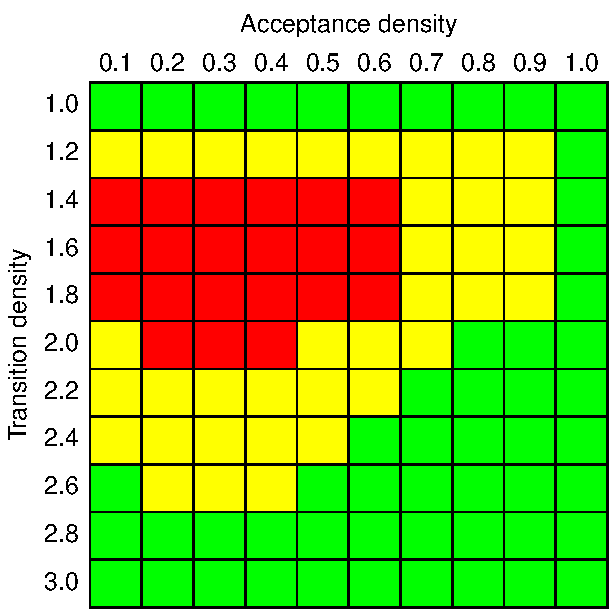
\includegraphics[width=0.35\textwidth]{figures/r/internal/goal/difficulty.pdf}
\caption{Difficulty categories \textit{easy} (green), \textit{medium} (yellow), and \textit{hard} (red) of the 110 transiton density/acceptance density classes of the \goal{} test set.}
\label{i.g.difficulty}
\end{figure}

Figure~\ref{i.g.difficulty}, shows a total of  53 easy, 36 medium, and 21 hard classes. The easy classes are mainly those with extreme values. All the classes with a transition density of 0.1, or 2.8 and 3.0, and a high acceptance density of 1.0 are easy. Furthermore, there is a ``triangle'' of easy classes between transition densities 2.0 and 2.6. and acceptance densities 0.5 and 0.9. The lower the transition density, the higher the acceptance density must be such that the class is classified as easy. The hard classes are roughly those with a transition density between 1.4 and 1.8 and an acceptance density between 0.1 and 0.6. The medium classes finally are located as a ``belt'' around the hard classes.

It is interesting to see that the hard automata are those with a ``medium'' transition density between 1.4 and 1.8. This range of transition densities means that every state has on average 1.4 to 1.8 outgoing transitions for each symbol of the alphabet. Somehow this specific level of connectivity seems to make the complementation of an automaton very hard. If the connectivity is lower, complementation becomes easier, and if the connectivity is harder, complementation becomes easier as well. A reason that complementation becomes easier with a lower transition density might be that such automata may contain unreachable and disconnected state. We let further investigations on the influence of the transiton density on the complementation difficulty for future work.

Figure~\ref{i.g.difficulty} also shows that automata with a larger number of accepting states are generally easier to complement. This proposition has been made by Tsai et al.~\cite{2011_tsai}, and it is the base of the MACC option of many complementation construction in \goal{} (see Section~\ref{4_goal}). Summarising, we can say that a transition density between 1.4 and 1.8 makes automata hard to complement, but that this difficulty is alleviated by an increasing acceptance density.

Note that these results are specific to the Fribourg construction, and cannot be readily generalised to other constructions. Furthermore the results are based exclusively on the \goal{} test set with its specific types of automata. However, as we will see in the results of the external tests in Section~\ref{5_external_goal}, other complementation constructions show a similar behaviour on the automata of the \goal{} test set.

% It is interesting that the extreme values of transition and acceptance densities result in easy automata. With a transition density of 1.0 and an alphabet size of 2, each of the 15 states has on average two outgoing and two incoming transitions. With a transition density of 3.0, each state has on average 6 outgoing and 6 incoming transitions. These low or high connectivity seems to considerably simplify the complementation task. The same applies to a high acceptance density of 1.0, which means that every state is an accepting state.

% Generally, we can say that automata with high acceptance densities are easier to complement than automata with lower acceptance densities. This also means that the pattern of easy automata at the extreme values of transition and acceptance density, does not apply to to the lower extreme of the acceptance density. Automata with a very low acceptance density of 0.1 are hard to complement---unless they are made easy by a low or high transition density.

% Another interesting point is that the hard automata have transition densities between 1.4 and 1.8. It seems that this range of transition densities is the crucial factor in the hardness of a complementation task, and that it is only alleviated by a growing acceptance density. This explains the decline of the mountain ridge from low to high acceptance density values.

% Summarising we can say that transition densities between 1.4 and 1.8 produce the hardest complementation tasks, and that to the both sides the difficulty steadily decreases with declining or growing transition density. Furthermore, a growing acceptance density generally implies easier complementation tasks.


\subsection{Michel Test Set}
\label{5_internal_michel}
The Michel test set consists of the four Michel automata Michel~1, Michel~2, Michel~3, and Michel~4 (characterised by the coefficient $m=\{1,2,3,4\}$) that are shown in Figure~\ref{4_michel_automata}. These automata have 3, 4, 5, and 6 states, respectively. The versions of the Fribourg constrcution that we tested on the Michel test set are the following (see Section~\ref{4_internal}):

\begin{enumerate}
\item Fribourg
\item Fribourg+R2C
\item Fribourg+M1
\item Fribourg+M1+M2
\item Fribourg+M1+M2+R2C
\item Fribourg+R
\end{enumerate}

In Table~\ref{i.m.states}, we present the complement sizes of these versions on the four Michel automata. The column \textit{Fitted curve} contains a function of the form $(an)^n$ that we fitted onto the four $xy$-points of each construction, where the $x$-axis is represents the size of the input automata (in our case 3, 4, 5, and 6), and the $y$-axis represents the size of the corresponding complements. The used fitting method was the method of non-linear least squares. The column \textit{Std. error} shows the standard error that resulted from the fit.

\begin{table}[htb]
\centering
% latex table generated in R 3.1.2 by xtable 1.7-4 package
% Sun Aug 16 00:19:45 2015
\begin{tabular}{lrrrrrr}
  \hline
Construction & Michel 1 & Michel 2 & Michel 3 & Michel 4 & Fitted curve & Std. error \\ 
  \hline
Fribourg & 57 & 843 & 14,535 & 287,907 & $(1.35n)^n$ & 0.01\% \\ 
  Fribourg+R2C & 33 & 467 & 8,271 & 168,291 & $(1.24n)^n$ & 0.06\% \\ 
  Fribourg+M1 & 44 & 448 & 5,506 & 81,765 & $(1.10n)^n$ & 0.07\% \\ 
  Fribourg+M1+M2 & 42 & 402 & 4,404 & 57,116 & $(1.03n)^n$ & 0.12\% \\ 
  Fribourg+M1+M2+R2C & 28 & 269 & 3,168 & 43,957 & $(0.99n)^n$ & 0.04\% \\ 
  Fribourg+R & 18 & 95 & 528 & 3,315 & $(0.64n)^n$ & 0.35\% \\ 
   \hline
\end{tabular}

\caption{Complement sizes of the Michel automata 1 to 4 ($m=\{1,2,3,4\}$), which have 3, 4, 5, and 6 states, respectively. }
\label{i.m.states}
\end{table}

% In the second-last column ``Fitted curve'' of Table~\ref{i.m.states}, we fitted a function of the form $(an)^n$ to the measured four data points. These data points consist of the sizes of the four Michel automata (3, 4, 5, and 6) as the $x$-values ad the corresponding complement sizes as the $y$-values. The fitted function $(an)^n$ can be seen as an ``averaged'' state growth of these four automata ($n$ is the size of the input automaton). The last column ``Std. error'' contains the standard error that resulted from the fit.

We can see in Table~\ref{i.m.states} that the state growths are indeed very large. For example, complementing Michel~4, which has six states, with the plain Fribourg construction results in a complement of 287,907 states. However, the optimisations R2C, M1, and M2 have a large influence on the complement sizes. If we consider Michel~4, then the R2C optimisation alone reduces the complement size from 287,907 to 168,291 which is a reduction of 51.5\%. The M1 optimisation has an eve larger influence as it reduces the complement size from 287,907 to 81,765 which is a reduction of 71.6\%. Adding M2 to M1 further reduces the complement size of Fribourg+M1 by 30.1\% (from 81,765 to 57,116). Finally, adding R2C on top of M1 and M2 brings a further reduction of of 23\% (from 57,116 to 43,957). If we compare the most efficient version (Fribourg+M1+M2+R2C) with the least efficient one (Fribourg), then the complement size of the former version is only 15.3\% of the complement size of the latter version.

It is interesting to see that for the Michel automata Fribourg+M1+M2 is more efficient than Fribourg+M1. For the \goal{} test set, Friburg+M1+M2 had a slightly higher median than Fribourg+M1 although it had a slightly lower mean. We identified in Section~\ref{5_internal_goal} that the M2 optimisation has a positive effect only on some automata, and that these are mostly the hard automata \textcolor{red}{(The automata with acceptance densities up to 0.4)}. Michel automata are very hard automata \textcolor{red}{(The acceptance densities of the four tested Michel automata are 0.25 or less)}, and indeed the M2 optimisation has a considerably positive effect. These results support thus the observation we made in Section~\ref{5_internal_goal}.

The special version Fribourg+R yields very small complements compared to the other versions. This tells us that the complements of the other versions contain a large number of unreachable and dead states. For example, the complement of Michel~4 of Fribourg+R (3,315 states) is 1.2\% of the size of the complement of Fribourg. This means that 98.8\% of the 287,907 states of the complement of Fribourg are unreachable and dead states. This is actually not surprising, because, following the proof of Michel~\cite{michel1988}\cite{1996_thomas}, the smallest possible complement of Michel~4 has 24 states. This is because Michel~4 has $m=4$ and Michel proved that the complement has at least size $m!$. This means that that even after reducing all the unreachable and dead states from the complement of Fribourg, an even much smaller complement would still be possible.

Up to now we just looked at the specific results of Michel~4. The fitted functions of the form $(an)^n$ summarise the results of all the four Michel automata. These functions give us reference points for the worst-case state complexities of the different versions of the Fribourg construction. For example, for the plain Fribourg construction with its fitted function of $(1.35n)^n$, we have now the proof that this construction produces complements of size $(1.35n)^n$, where $n$ is the size of the input automaton. This means that the worst-case complexity cannot be lower than $(1.35n)^n$ (but it can still be higher). This bound decreases for the different versions of the Fribourg construction down to $(0.99n)^n$ for Fribourg+M1+M2+R2C.

In Table~\ref{i.m.times} we show the measured execution time in seconds (CPU time) for each complementation task. We can see that the difference between the least and most efficient version is bigger than for the complement sizes. For example for Michel~4, Fribourg+M1+M2+R2C is more than 43 times faster than Fribourg (2,332.6 seconds compared to 100,976 seconds). In more familiar unities, this corresponds to approximately 39 minutes for Fribourg+M1+M2+R2C against 28 hours for Fribourg. We also fitted functions of the form $(an)^n$ to the measured execution times where $n$ is the number of states of the input automaton, and the value of the function is the execution time of the task in CPU time seconds.

\begin{table}[htb!]
\centering
% latex table generated in R 3.1.2 by xtable 1.7-4 package
% Sun Aug 16 16:21:25 2015
\begin{tabular}{lrrrrrr}
  \hline
Construction & Michel 1 & Michel 2 & Michel 3 & Michel 4 & Fitted curve & Std. error \\ 
  \hline
Piterman+EQ+RO & 2.5 & 3.8 & 42.6 & 75,917.4 & $(1.08n)^n$ & 0.64\% \\ 
  Slice+P+RO+MADJ+EG & 2.3 & 3.6 & 11.4 & 159.5 & $(0.39n)^n$ & 0.38\% \\ 
  Rank+TR+RO & 2.2 & 3.0 & 6.4 & 30.0 & $(0.29n)^n$ & 0.18\% \\ 
  Fribourg+M1+M2+R2C & 2.5 & 3.5 & 10.8 & 2,332.6 & $(0.61n)^n$ & 0.62\% \\ 
   \hline
\end{tabular}

\caption{Execution time in seconds (CPU time) for complementing the Michel automata~1 to~4.}
\label{i.m.times}
\end{table}

The fitted functions that we calculated for the measured complement sizes and execution times are based on only four data points. This is generally not enough to make reliable extrapolations. However, it is still interesting to do such an extrapolation in order to see the involved complexity and to show why we were restricted to include only the first four Michel automata in the test set. In Table~\ref{i.m.extrapolation}, we show extrapolated values for the complement sizes and execution times for the plain Fribourg construction (the least efficient one), based on the corresponding fitted functions. The table includes the extrapolated values for the Michel automata 5 to 8, which have 7 to 10 states. 


\begin{table}[htb]
\centering
\begin{tabular}{lrrrr}
\hline
Automaton & States ($n$) & Compl. size $(1.35n)^n$ & Exec. time $(1.14n)^n$ & $\approx$ days/months/years \\
\hline
Michel 5 &  7 &       6,882,980 &      2,020,385 &     23 days   \\
Michel 6 &  8 &     189,905,394 &     46,789,245 &     18 months \\
Michel 7 &  9 &   5,939,189,262 &  1,228,250,634 &     39 years  \\
Michel 8 & 10 & 207,621,228,081 & 36,039,825,529 &  1,142 years  \\
\hline
\end{tabular}
\caption{Extrapolated values for the complement sizes and execution times (seconds CPU time)  for the Michel automata with $m=\{5,\dots,10\}$ with the Fribourg version of the Fribourg construction.}
\label{i.m.extrapolation}
\end{table}

According to the fitted state growth function, the complement of Michel~5 would have nearly 7 million states, and the complement of Michel~8 even more than 207 billion states. Already the computation of the 7 million states of Michel~5 would most probably exceed the available memory resources in our computing environment. Regarding execution time, the complementation of Michel~5 would take 23 days. This would by far exceed the maximal running time of a job on our computer cluster. And even if we would not have these administrative time restriction, the time to wait for the complementation of Michel~5 to~8, between 18 months and 1,142 years, is definitely too long, even for a master's thesis.


\section{Results of the External Tests}
\label{5_external}
In the external tests we compared the most efficient version of the Fribourg construction to three other constructions. These constructions are Piterman+EQ+RO, Slice+P+RO+MADJ+EG, and Rank+TR+RO. The most efficient version of the Fribourg construction is Fribourg+M1+R2C for the \goal{} test set, and Fribourg+M1+M2+R2C for the Michel test set. We present the results from these two test sets separately in the following two sections.


\subsection{GOAL Test Set}
\label{5_external_goal}
As for the internal tests on the \goal{} test set, we set a time limit of 600 seconds CPU time, and a Java heap size limit of 1 GB per complementation task.  Table~\ref{e.g.outs} shows the number of timeouts and memory excesses that we observed for the four constructions.

\begin{table}[ht]
\centering
% latex table generated in R 3.1.2 by xtable 1.7-4 package
% Sat Jun  6 16:42:17 2015
\begin{tabular}{lrr}
  \hline
Construction & Timeouts & Memory excesses \\ 
  \hline
Fribourg & 48 & 0 \\ 
  Fribourg+R2C & 30 & 0 \\ 
  Fribourg+R2C+C & 54 & 0 \\ 
  Fribourg+M1 & 2 & 0 \\ 
  Fribourg+M1+M2 & 1 & 0 \\ 
  Fribourg+M1+R2C & 1 & 0 \\ 
  Fribourg+M1+R2C+C & 8 & 0 \\ 
  Fribourg+R & 48 & 0 \\ 
   \hline
\end{tabular}

\caption{Number of timeouts and memory excesses for the \goal{} test set.}
\label{e.g.outs}
\end{table}

\subsubsection{With Rank}

Most salient in Table~\ref{e.g.outs} is the high number of aborted tasks for the Rank construction. 3,317 of the 11,000 automata (33.8\%) were aborted due to a timeout, and further 83 (0.8\%) due to a memory excess. Regarding the other constructions, there are just two timeouts for the Piterman construction, and a single timeout for the Fribourg construction.

Determining the effective samples of these runs gives a number of 7,204 automata, which is 65.5\% of the total number of automata. In Figure~\ref{e.g.stripchart.with_rank} we present the complement sizes of these 7,204 effective samples as a stripchart. 

\begin{figure}[ht]
\centering
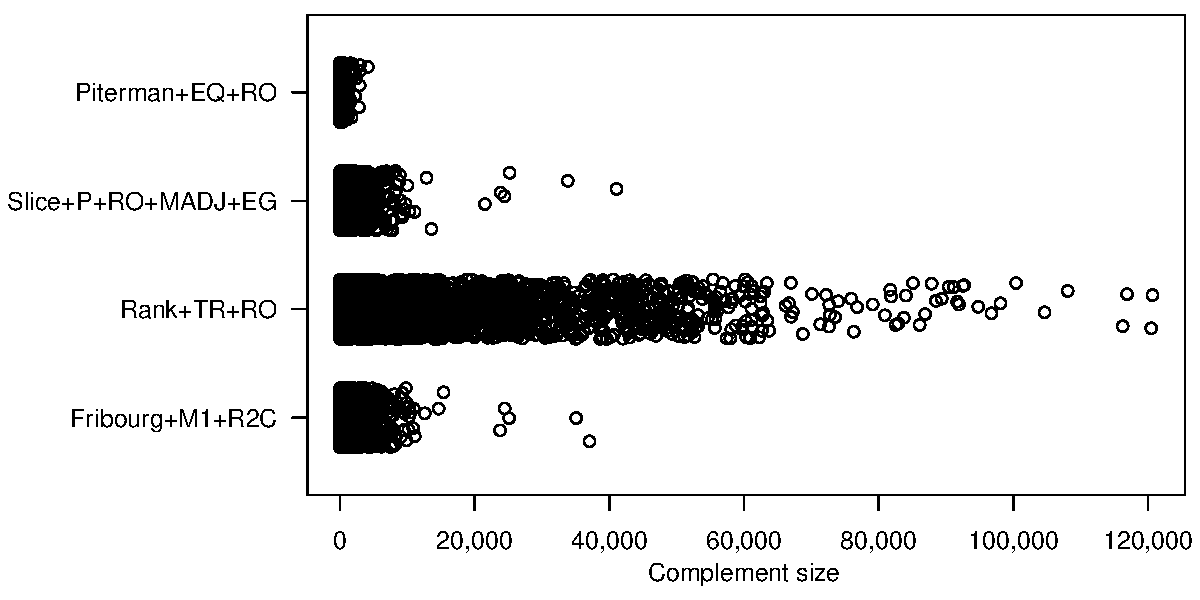
\includegraphics[width=0.75\textwidth]{figures/r/external/goal/s.stripchart.with_rank.pdf}
\caption{Complement sizes of the 7,204 effective samples.}
\label{e.g.stripchart.with_rank}
\end{figure}

The stripchart makes the reason for the high number of aborted tasks of the Rank construction apparent. Rank+TR+RO produces a high number of very large complements compared to the other constructions.

But from the stripchart in Figure~\ref{e.g.stripchart} alone we cannot yet tell whether the Rank construction \textit{generally} produces larger complements than the other constructions, or if this holds just for \textit{some} automata. To this end we have to inspect the statistics about the distribution of the complement sizes in Table~\ref{e.g.stats.with_rank}.

\begin{table}[ht]
\centering
% latex table generated in R 3.1.2 by xtable 1.7-4 package
% Sun Aug 16 15:57:19 2015
\begin{tabular}{lrrrrrr}
  \hline
Construction & Mean & Min. & P25 & Median & P75 & Max. \\ 
  \hline
Piterman+EQ+RO & 106.0 & 1 & 29.0 & 58.0 & 121.0 & 4,126 \\ 
  Slice+P+RO+MADJ+EG & 555.4 & 2 & 70.0 & 202.0 & 596.0 & 41,081 \\ 
  Rank+TR+RO & 5,255.6 & 2 & 81.0 & 254.5 & 3,178.2 & 120,674 \\ 
  Fribourg+M1+R2C & 662.9 & 2 & 101.0 & 269.0 & 754.5 & 37,068 \\ 
   \hline
\end{tabular}

\caption{Statistics of complement sizes of the 7,204 effective samples}
\label{e.g.stats.with_rank}
\end{table}

And indeed, the 25th percentile and the median of Rank are higher than for Piterman and Slice, but still lower than for our Fribourg construction. This means that the Rank construction produces more smaller complements than the Fribourg construction. However, the picture changes dramatically for the 75th percentile where the value of Rank is more than four times higher than the value for Fribourg. Also the mean of Rank is many times higher than the means of all the other constructions. A possible explanation for this is that the Rank construction has a comparable performance with the other constructions for easy automata. For harder automata, however, the performance of Rank is much worse than the other constructions. In addition, the automata that are hardest for Rank are not even included in this analysis as it includes only the 7,204 effective samples. The 3,796 automata that are excluded would probably have resulted in even larger complements with the Rank construction.

What we cannot tell is whether the automata which are hard for Rank are the same that are hard for the other constructions. However, as we will see later, we think that this is not necessarily the case.

\subsubsection{Without Rank}

Given the large number of aborted complementation tasks of Rank we decided to do the main analysis and comparison of the results without the Rank construction. Because with the Rank construction would basically exclude more than one third of the tasks that have been successfully completed by the other constructions from the result analysis. Our main interest is however to compare the performance of the Fribourg construction to the other constructions. In this way, we would probably miss important aspects in the result analysis of the other three constructions. 

Without the Rank construction there are 10,998 effective samples In Figure~\ref{e.g.stripchart} we display the complement sizes of these 10,998 effective samples as a stripchart.

\begin{figure}[ht]
\centering
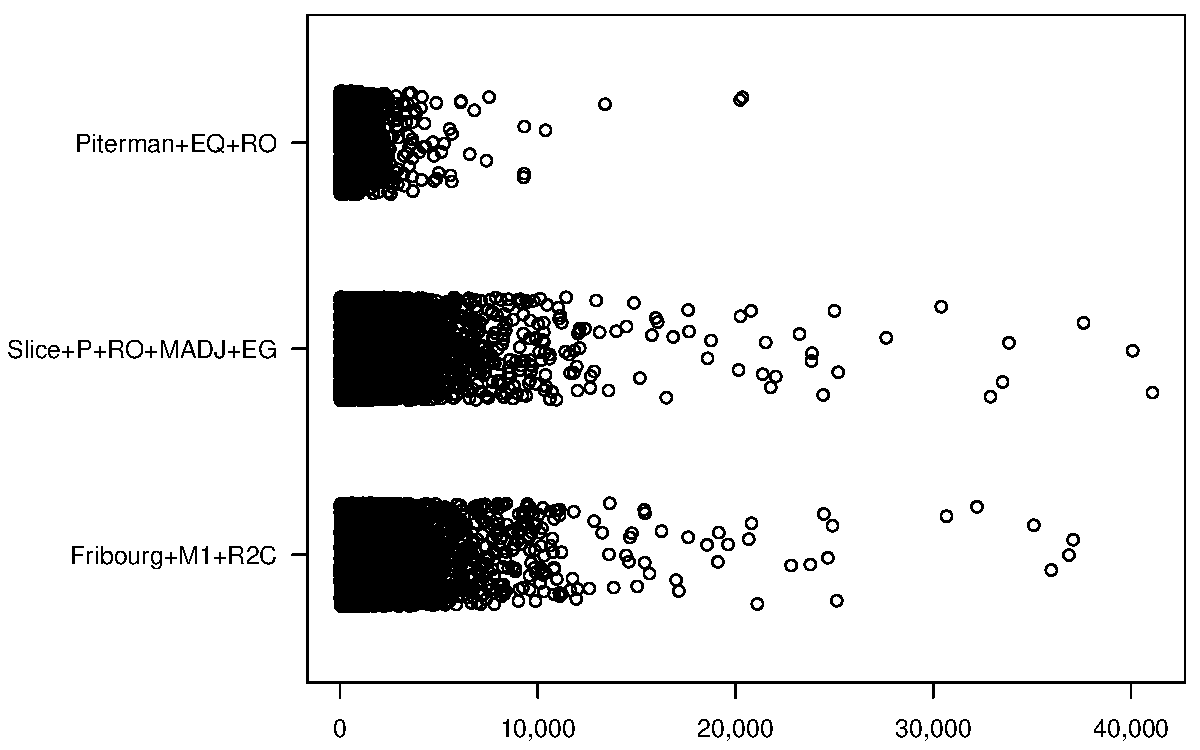
\includegraphics[width=0.75\textwidth]{figures/r/external/goal/s.stripchart.pdf}
\caption{Complement sizes of the 10,998 effective samples.}
\label{e.g.stripchart}
\end{figure}

From the stripchart we can see that Fribourg and Slice have a comparable distribution of complement sizes, whereas Piterman has a considerably higher concentration of small complement sizes. We can say that Piterman generally produces smaller complement than Fribourg and Slice.

We present the statistics of these distributions in Table~\ref{e.g.stats}. 
Indeed, for all statistics Piterman has values that are multiple times lower than the ones of Fribourg and Slice. It is interesting that for mean, 25th percentile, median, and 75th percentile the values of Piterman are more or less five times smaller. It seems like Piterman would produce complements that are throughout five times smaller than the complements of Fribourg and Slice.

\begin{table}[ht]
\centering
% latex table generated in R 3.1.2 by xtable 1.7-4 package
% Sat Jun  6 16:42:20 2015
\begin{tabular}{lrrrrrr}
  \hline
Construction & Mean & Min. & P25 & Median & P75 & Max. \\ 
  \hline
Piterman+EQ+RO & 209.6 & 1 & 38.0 & 80.0 & 183.0 & 20,349 \\ 
  Slice+P+RO+MADJ+EG & 949.4 & 2 & 120.0 & 396.0 & 1,003.0 & 41,081 \\ 
  Fribourg+M1+R2C & 1,017.3 & 2 & 153.0 & 452.0 & 1,134.0 & 37,068 \\ 
   \hline
\end{tabular}

\caption{Aggregated statistics of complement sizes of the 10,998 effective samples without Rank.}
\label{e.g.stats}
\end{table}

Comparing Fribourg and Slice, there is a slight advantage for Slice. Mean, 25th percentile, median, and 75th percentile are lower for Slice than for Fribourg by 6.7\%, 21.6\%, 12.4\%, and 11.6\%, respectively. We have to conclude that from an overall point of view, the Fribourg construction has the second-worst performance for the \goal{} test set after Piterman and Slice, and before Rank.

Figure~\ref{e.g.persp} shows the perspective plots with the median complement sizes for the 110 classes of the 10,998 samples. As already mentioned, the corresponding matrices can be found in Appendix~\ref{app_matrices}.


\renewcommand{\perspwidth}{0.3}
\begin{figure}[ht]
\centering
  \hfill
  \begin{subfigure}[t]{\perspwidth\textwidth}
  \centering
  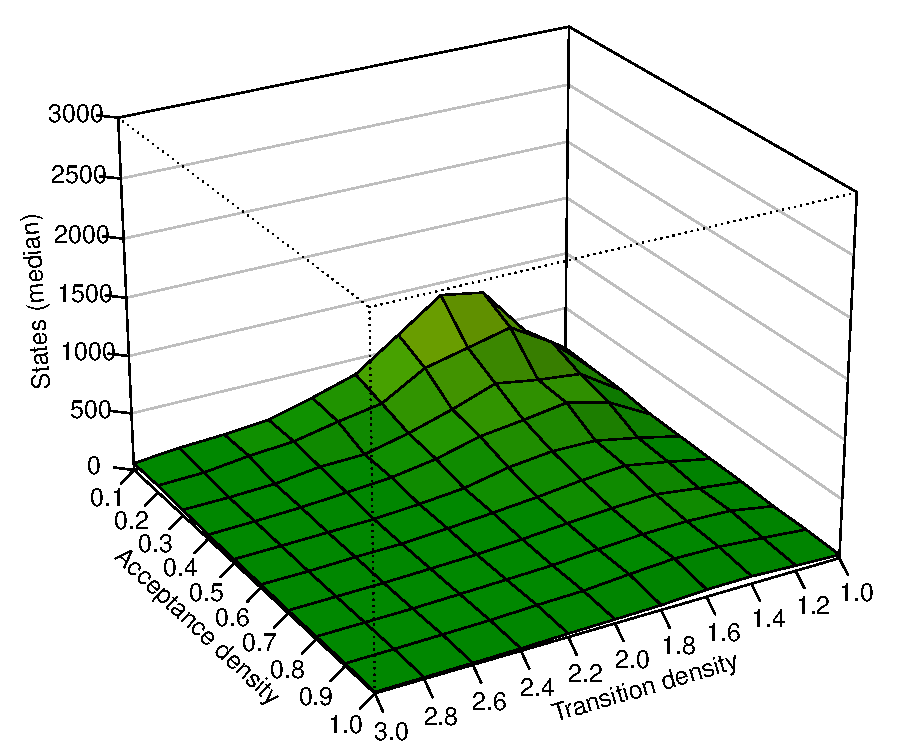
\includegraphics[width=\textwidth]{figures/r/external/goal/s.median.Piterman+EQ+RO.pdf}
  \caption{Piterman+EQ+RO}
  \end{subfigure}
  \hfill
  \begin{subfigure}[t]{\perspwidth\textwidth}
  \centering
  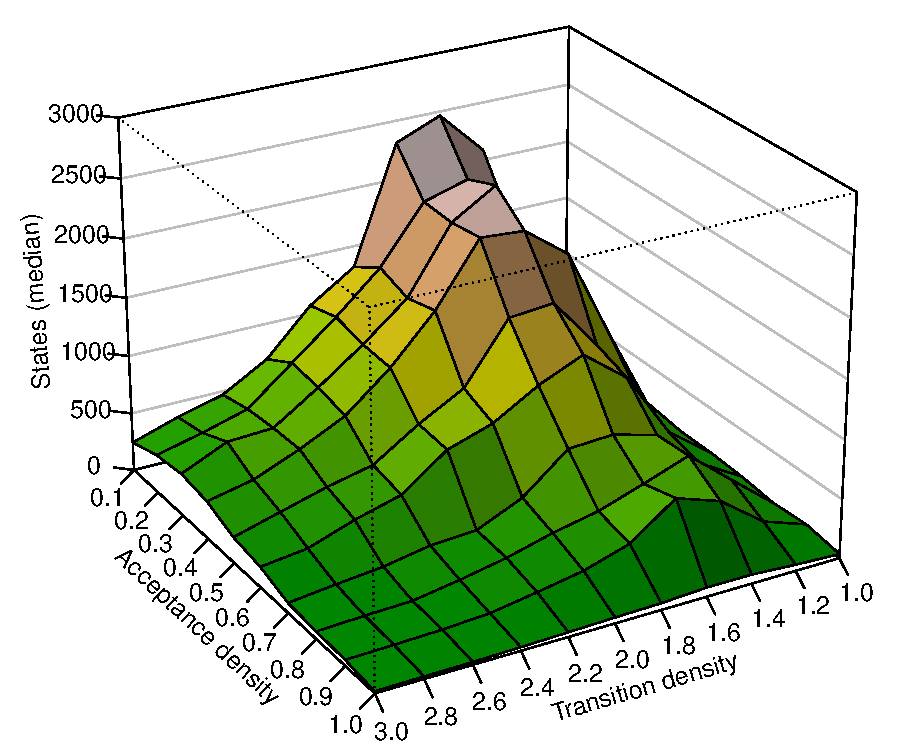
\includegraphics[width=\textwidth]{figures/r/external/goal/s.median.Slice+P+RO+MADJ+EG.pdf}
  \caption{Slice+P+RO+MADJ+EG}
  \end{subfigure}
  \hfill
  \begin{subfigure}[t]{\perspwidth\textwidth}
  \centering
  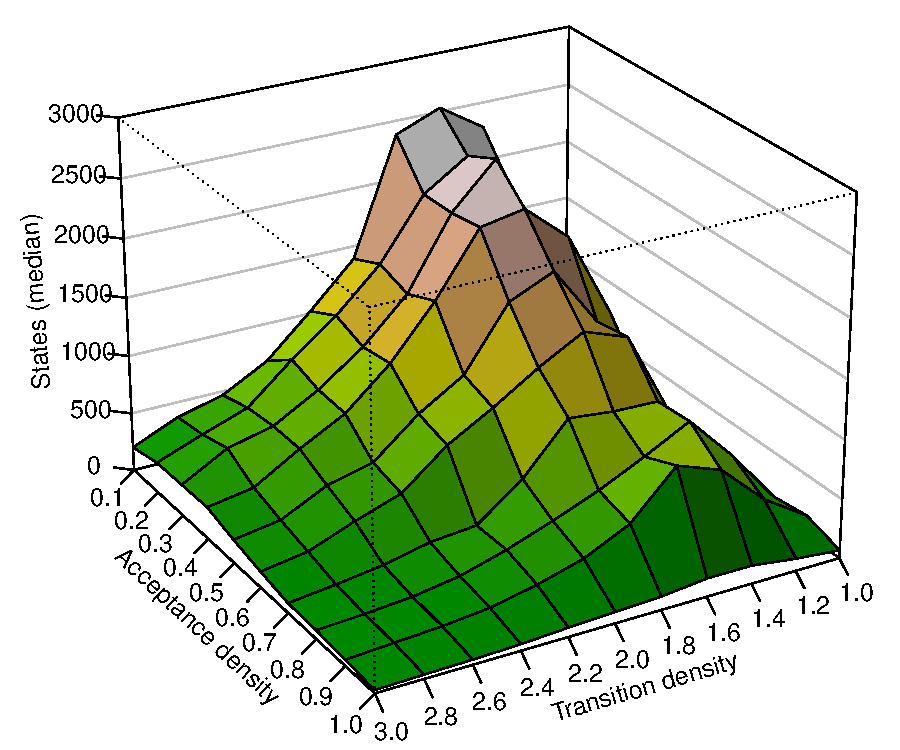
\includegraphics[width=\textwidth]{figures/r/external/goal/s.median.Fribourg+M1+R2C.pdf}
  \caption{Fribourg+M1+R2C}
  \end{subfigure}
  \hfill
\caption{Median complement sizes (10,998 samples)}
\label{e.g.persp}
\end{figure}

Note that the plot of Fribourg+M1+R2C in Figure~\ref{e.g.persp} (c) is the same as the one in Figure~\ref{i.g.persp_2} (b). The only difference is the scale of the vertical axis.

In the perspective plots we can see that the pattern for Fribourg and Slice are very similar. The median complement sizes in the individual classes do not differ a lot, both relatively and absolutely. However, the medians of Fribourg seem to be throughout (with some exceptions) slightly higher than the ones of Slice. This means that Fribourg and Slice seem to have similar strengths and weaknesses, but Slice is slightly more efficient on the tested automata.

Piterman, as expected, has medians that are multiple times lower than the corresponding medians of Fribourg and Slice. The basic pattern, however, is still similar. There is a mountain ridge along the classes with a transition density of 1.6 with its top in the class with transition density 1.6 and acceptance density 0.1.


\subsection{Michel Test Set}
\label{5_external_michel}
For the Michel test set we used the same three third-party construction as for the \goal{} test set, namely Piterman+EQ+RO, Slice+P+RO+MADJ+EG, and Rank+TR+RO. The used Fribourg construction version is however Fribourg+M1+M2+R2C, as this is the most efficient version of the Fribourg construction on the Michel test set.

The resulting complement sizes are shown in Table~\ref{e.m.states}. Again, we fitted a function of the form $(an)^n$ to the four measured data points of each construction and calculated the standard error of this fit.

\begin{figure}[ht]
\centering
% latex table generated in R 3.1.2 by xtable 1.7-4 package
% Sun Aug 16 00:19:45 2015
\begin{tabular}{lrrrrrr}
  \hline
Construction & Michel 1 & Michel 2 & Michel 3 & Michel 4 & Fitted curve & Std. error \\ 
  \hline
Fribourg & 57 & 843 & 14,535 & 287,907 & $(1.35n)^n$ & 0.01\% \\ 
  Fribourg+R2C & 33 & 467 & 8,271 & 168,291 & $(1.24n)^n$ & 0.06\% \\ 
  Fribourg+M1 & 44 & 448 & 5,506 & 81,765 & $(1.10n)^n$ & 0.07\% \\ 
  Fribourg+M1+M2 & 42 & 402 & 4,404 & 57,116 & $(1.03n)^n$ & 0.12\% \\ 
  Fribourg+M1+M2+R2C & 28 & 269 & 3,168 & 43,957 & $(0.99n)^n$ & 0.04\% \\ 
  Fribourg+R & 18 & 95 & 528 & 3,315 & $(0.64n)^n$ & 0.35\% \\ 
   \hline
\end{tabular}

\caption{Complement sizes of the first four Michel automata.}
\label{e.m.states}
\end{figure}

Considering the results of the \goal{} test set, the results in Table~\ref{e.m.states} are surprising. Rank is the most efficient construction. It produces the smallest complements for all Michel automata, and with $(0.91n)^n$ it has the flattest fitted curve of all constructions. This is surprising because for the \goal{} test set, Rank produced by far the largest complements, and 34.5\% of the test data could not even be completed within the given time and memory limits. With the Michel automata, however, the case seems to be reversed and Rank produces by far the smallest complements.

Rank is followed by the Fribourg construction, which has the second-smallest complements for Michel~3 and~4, and with $(0.99n)^n$ the second-flattest fitted curve. The complements of Michel~2, 3, and~4 of the Fribourg construction are bigger than the ones of the Rank construction by 48.6\%, 68.2\%, and 69.2\%, respectively.

The construction with the next steeper fitted curve of $(1.18n)^n$ is the Slice construction. for Michel~1 to~3, this is actually the worst construction, but then for Michel~4, the complement is smaller than the one of Piterman what results in the flatter fitted curve. The gap to the Fribourg construction is big. The complement sizes of Michel~2 to~4 exceed the ones of Fribourg by 60.2\%, 114.2\%, and 180.2\%, respectively. This is also a remarkable point, because for the \goal{} test set, Fribourg and Slice showed a very similar performance.

The last in the ranking is Piterman with a fitted curve of $(1.25n)^n$. However, a special fact for Piterman is that it has the smallest complement for Michel~1 (together with Rank), the second-smallest for Michel~2, the third-smallest for Michel~3, and the largest for Michel~4. It is actually the large complement of Michel~4 that makes Piterman having the steepest fitted curve. However, it is still remarkable that this construction, which is by far the most efficient for the \goal{} test set, produces so much worse results for the Michel automata than all the other constructions. Compared with the Rank construction, Piterman's complements of Michel~2 to~4 are 38.7\%, 174.3\%, and 573.6\%, respectively, bigger. Compared to the Fribourg construction, Piterman produces slightly smaller complements for Michel~1 and~2, but larger ones for Michel~3 and~4. Namely, they are 63.1\% and 298.2\% larger than the corresponding ones of the Fribourg construction.

Summarising we can say that the ranking of the constructions for the Michel test set is exactly the reverse of the ranking for the \goal{} test set. The by far worst construction for the \goal{} test set (Rank) is the best one for the Michel test set, and the by far best construction for the \goal{} test set (Piterman) is the worst one for the Michel test set (at least for Michel~4). For the Fribourg construction this means that it ``advances'' from rank 3 for the \goal{} test set to rank 2 for the Michel test set.

In Table~\ref{e.m.times} we present the execution times per complementation task in CPU time seconds. As for the complement sizes, we fitted a function of the form $(an)^n$ to the measured execution times where $n$ is the size of the input automaton.

\begin{table}[ht]
\centering
% latex table generated in R 3.1.2 by xtable 1.7-4 package
% Sun Aug 16 16:21:25 2015
\begin{tabular}{lrrrrrr}
  \hline
Construction & Michel 1 & Michel 2 & Michel 3 & Michel 4 & Fitted curve & Std. error \\ 
  \hline
Piterman+EQ+RO & 2.5 & 3.8 & 42.6 & 75,917.4 & $(1.08n)^n$ & 0.64\% \\ 
  Slice+P+RO+MADJ+EG & 2.3 & 3.6 & 11.4 & 159.5 & $(0.39n)^n$ & 0.38\% \\ 
  Rank+TR+RO & 2.2 & 3.0 & 6.4 & 30.0 & $(0.29n)^n$ & 0.18\% \\ 
  Fribourg+M1+M2+R2C & 2.5 & 3.5 & 10.8 & 2,332.6 & $(0.61n)^n$ & 0.62\% \\ 
   \hline
\end{tabular}

\caption{Execution times for the first four Michel automata.}
\label{e.m.times}
\end{table}

Most interesting in Table~\ref{e.m.times} is the column with the times for Michel~4. The time difference between the best and the worst construction is enormous. While the Rank construction took just 30 seconds to complement Michel~4, the Piterman construction took 75,917.4 seconds which is approximately 21 hours. This is more than 2500 times longer. Of course the Piterman construction produced a bigger automata, which naturally requires more time, however, the automaton produced by the Piterman construction is just around 6.7 times bigger than the one of the Rank construction. This means that the Piterman construction must include very inefficient processes before finally arriving at the output automaton.

Furthermore, we can see in Table~\ref{e.m.times} that also the Fribourg construction took relatively long to complement Michel~4 compared to Rank, namely 2,332.6 seconds which are approximately 39 minutes. This is 77.8 times longer than the 30 seconds of Rank. At the same time, Fribourg's complement has just 68.2\% more states than Rank's complement. Similarly, compared to the Slice construction the Fribourg construction is slow for Michel~4. Slice's complement is 2.8 times bigger than Fribourg's complement, but with 159.5 seconds the complementation of slice was 14.6 times faster than the complementation of Fribourg.

So there seems to an inefficiency in the Fribourg construction in terms of execution time for the complementation of Michel~4. However, this inefficiency is by far not as pronounced as for Piterman. While the complement of Piterman is just 4 times bigger, the execution time of Piterman is 32.5 times longer than the one of the Fribourg construction. One could also look at it from the other side and say that not the Fribourg construction is inefficient on Michel~4, but that Rank and Slice are extremely efficient on this automaton.

Finally, these interesting differences in the execution times between the four constructions can only be observed for Michel~4. For Michel~3 there are also differences but they are by far not as pronounced as for Michel~4. If the computational resources would allow it, it would be very interesting to run the constructions on Michel~5 and beyond. One thing that stays the same for all the four Michel automata is that Rank is always the fastest and Piterman always the slowest construction.

\section{Discussion}
\label{5_discussion}

\subsection{Sumary of the Results}
\label{5_summary}

\subsection{Limitations of the Study}
\label{5_limitations}
